\section{Target Outputs: Worked Examples and Coverage Analysis}
\label{sec:target-outputs}

This section validates the Timeline Compiler design against five concrete end-results
provided by the project owner. For each target we embed the reference image, characterise
the visual, prove representability with a worked Timeline IR in YAML using Mark's field
names (Section~\ref{sec:ir}), and state the layout family, theme, effects, and backend
tier required. Section~\ref{sec:target-synthesis} then synthesises the findings: new layout
families the targets demand, a consolidated coverage table, a structured gap list, and a
prioritised verdict.

%% ============================================================================
%% T1
%% ============================================================================
\subsection{T1 --- Vertical Spine, Dark Theme, Icon Badges}
\label{sec:target-t1}

\begin{figure}[ht]
\centering
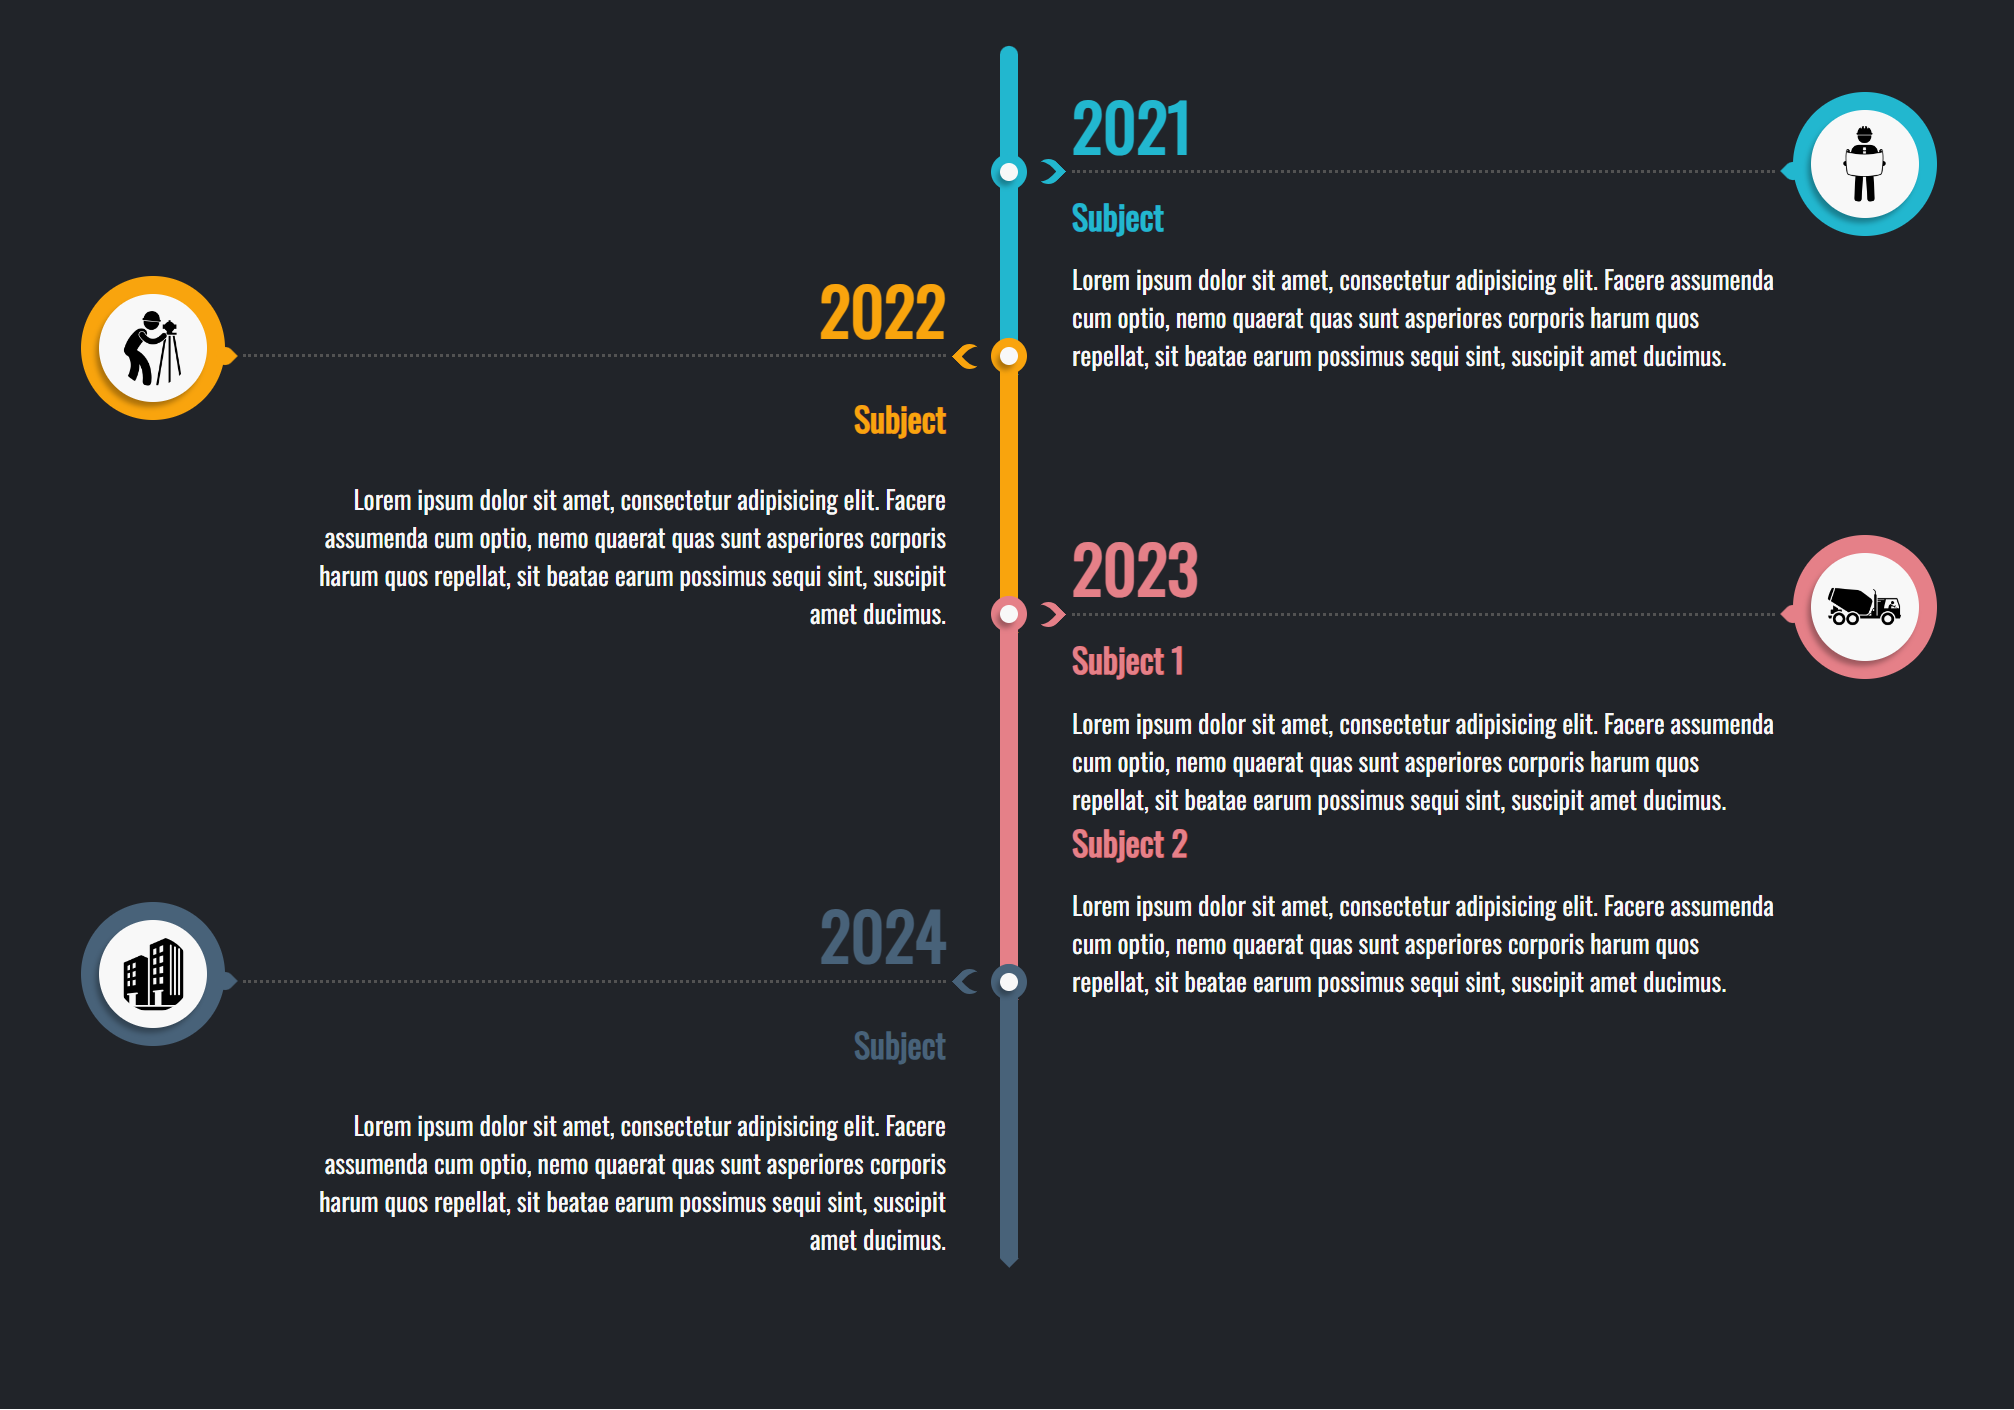
\includegraphics[width=\linewidth]{figures/target-vertical-spine-dark.png}
\caption{T1: Vertical central-spine timeline, dark charcoal background, colour-coded year
  segments, alternating left/right text entries, and circular icon badge callouts with
  dashed leader lines. (Reference image provided by project owner.)}
\label{fig:target1}
\end{figure}

\paragraph{Visual characterisation.}
\begin{itemize}
  \item \textbf{Layout family:} Vertical central-spine; time axis runs top to bottom; year
        nodes (small circles) sit on the spine; entries alternate right/left by year.
  \item \textbf{Spine segmentation:} Each year-to-year segment is coloured distinctly:
        cyan (2021), amber (2022), pink--red (2023), slate-blue (2024).
  \item \textbf{Entry style:} Coloured ``Subject'' heading plus body paragraph, stacked
        left or right of the node. Year 2023 has \emph{two} stacked subjects under one
        node.
  \item \textbf{Icon badges:} Circular white disc with coloured ring and soft drop shadow,
        holding pictograms (hard-hat worker, surveyor, cement truck, office building).
        Each badge sits at the far canvas edge, connected to its year node by a horizontal
        dashed leader line with a small arrowhead.
  \item \textbf{Theme/mood:} Dark charcoal background, clean sans-serif, soft shadows,
        high contrast colour accents.
\end{itemize}

\paragraph{Worked Timeline IR.}
The year nodes map to \texttt{milestones}; each subject entry maps to an \texttt{activity}
with \texttt{span} equal to the relevant year. Two subjects in 2023 share a
\texttt{group}. Per-node colour is expressed via \texttt{category} resolved through the
theme's \texttt{category\_map} (the IR has no direct \texttt{color} field on milestones
or activities---see Gap~IR-2 in Section~\ref{sec:target-gaps-ir}). The icon pictogram is
carried by \texttt{milestone.icon}. Alternating side placement and the badge-leader-line
visual are render concerns, not IR data.

\begin{lstlisting}[language=yaml,caption={T1 worked IR --- vertical spine, dark, icon badges (abbreviated)}]
version: "1.0"
metadata:
  title: "Company Journey 2021-2024"
  today: 2026-06-10
  time_range:
    start: 2021
    end: 2024
  axis_unit: year
  theme: dark-executive          # GAP: theme does not yet exist (see Sec. 14.6c)
tracks:
  - id: spine
    label: ""
    index: 0
groups:
  - id: y2023-entries
    label: "2023"
    members: [y2023-s1, y2023-s2]
milestones:
  - id: y2021
    label: "2021"
    date: 2021-01-01
    track: spine
    icon: hard-hat-worker        # pictogram hint; renderer resolves to pictogram
    category: year-cyan          # theme category_map: { year-cyan: {fill: "#00BCBE"} }
  - id: y2022
    label: "2022"
    date: 2022-01-01
    track: spine
    icon: surveyor
    category: year-amber         # theme category_map: { year-amber: {fill: "#F5A623"} }
  - id: y2023
    label: "2023"
    date: 2023-01-01
    track: spine
    icon: cement-truck
    category: year-red           # theme category_map: { year-red: {fill: "#E8314A"} }
  - id: y2024
    label: "2024"
    date: 2024-01-01
    track: spine
    icon: office-building
    category: year-slate         # theme category_map: { year-slate: {fill: "#4A6FA5"} }
activities:
  - id: y2021-entry
    label: "Subject"
    track: spine
    span: 2021
    description: "Body text describing the 2021 period."
    category: year-cyan
    metadata:
      entry_side: right          # render hint: vertical-spine renderer reads this
  - id: y2022-entry
    label: "Subject"
    track: spine
    span: 2022
    description: "Body text describing the 2022 period."
    category: year-amber
    metadata:
      entry_side: left
  - id: y2023-s1
    label: "Subject 1"
    track: spine
    span: 2023
    group: y2023-entries
    description: "Body text for 2023 Subject 1."
    category: year-red
    metadata:
      entry_side: right
  - id: y2023-s2
    label: "Subject 2"
    track: spine
    span: 2023
    group: y2023-entries
    description: "Body text for 2023 Subject 2."
    category: year-red
    metadata:
      entry_side: right
  - id: y2024-entry
    label: "Subject"
    track: spine
    span: 2024
    description: "Body text describing the 2024 period."
    category: year-slate
    metadata:
      entry_side: left
# Icon badge leader lines: the vertical-spine renderer draws these automatically
# from each milestone icon badge to its spine node; badge position is a
# layout-family concern and requires no separate annotation in the IR.
\end{lstlisting}

\paragraph{IR field mapping summary.}
\texttt{milestones[].icon} carries the pictogram hint.
\texttt{milestones[].category} resolves to per-year spine colour via
\texttt{theme.category\_map}.
\texttt{activities[].group} clusters the two 2023 subjects.
The \texttt{entry\_side} key within \texttt{activities[].metadata} is a render hint read
by the vertical-spine layout module (open extension map; no IR schema change needed).
Multiple subjects under one node are fully expressible using \texttt{group.members}.

\paragraph{Layout, theme, effects, and tier.}
\begin{itemize}
  \item \textbf{Layout family:} Vertical central-spine with alternating card entries
        (Section~\ref{sec:target-layout-families}).
        \textbf{Gap Render-1}: not in current \S5 pipeline.
  \item \textbf{Theme:} Dark-executive --- deep charcoal background, coloured spine
        segments, drop-shadow icon badges. \textbf{Gap Theme-1}: no dark theme in the
        current five; see Section~\ref{sec:target-gaps-theme}.
  \item \textbf{Effects:} Drop shadow on icon badges (Tier~2 \texttt{DropShadow});
        dashed-leader connector style (annotation \texttt{connector\_style} vocabulary
        extension, Gap Render-5). Already supported by the effect registry
        (\S\ref{sec:schema-fidelity}).
  \item \textbf{Fidelity tier:} Tier~2 (Polished); SVG backend with safe-filter caveat
        or Raster backend. PPTX native \texttt{a:outerShdw} satisfies the drop-shadow.
\end{itemize}


%% ============================================================================
%% T2
%% ============================================================================
\subsection{T2 --- Horizontal Linear, Light, Numbered Nodes}
\label{sec:target-t2}

\begin{figure}[ht]
\centering
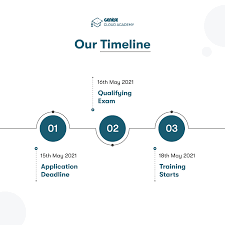
\includegraphics[width=\linewidth]{figures/target-horizontal-numbered.png}
\caption{T2: Horizontal single-line timeline, white background, three large numbered
  circular nodes (01/02/03), date above each node, title below. Corporate minimal
  aesthetic with generous whitespace. (Reference image provided by project owner.)}
\label{fig:target2}
\end{figure}

\paragraph{Visual characterisation.}
\begin{itemize}
  \item \textbf{Layout family:} Horizontal single-line; a single axis with no track
        swimlanes; milestones only, evenly spaced.
  \item \textbf{Node style:} Large filled circles in dark teal, with a bold ordinal
        number centred (01, 02, 03); the middle node is visually emphasised.
  \item \textbf{Labels:} Date string above each node (e.g., ``15th May 2021''); title
        below (Application Deadline / Qualifying Exam / Training Starts).
  \item \textbf{Theme/mood:} Light/white background; ``Our Timeline'' header with logo;
        minimal, corporate, generous whitespace; no decorative chrome.
\end{itemize}

\paragraph{Worked Timeline IR.}
This is the most directly representable target. A single empty track carries three
milestones; \texttt{metadata.title} is the header text. The ordinal number (01, 02, 03)
is \emph{purely a render concern}---the vertical-spine renderer assigns sequential
numbers by milestone sort order (\texttt{date\_ordinal, id}), so no IR field is needed.
The logo is a theme-level image asset. Emphasis on the middle node is a \texttt{tags}
hint or a theme-defined category.

\begin{lstlisting}[language=yaml,caption={T2 worked IR --- horizontal linear, numbered nodes (abbreviated)}]
version: "1.0"
metadata:
  title: "Our Timeline"
  today: 2026-06-10
  time_range:
    start: 2021-03
    end: 2021-11
  axis_unit: month
  theme: light-minimal-corporate  # GAP: theme does not yet exist (Sec. 14.6c)
  locale: en
tracks:
  - id: main
    label: ""
    index: 0
milestones:
  - id: app-deadline
    label: "Application Deadline"
    date: 2021-05-15
    track: main
    status: done
    category: standard-node
  - id: qualifying-exam
    label: "Qualifying Exam"
    date: 2021-06-20
    track: main
    status: in-progress
    tags: [emphasized]             # render hint: larger/filled node treatment
    category: standard-node
  - id: training-starts
    label: "Training Starts"
    date: 2021-09-01
    track: main
    status: planned
    category: standard-node
# Ordinal node numbers (01, 02, 03) are assigned by the renderer in
# milestone sort order; no IR field required.
# Logo in header: a theme asset, not IR data.
\end{lstlisting}

\paragraph{IR field mapping summary.}
\texttt{milestones[].label} becomes the title below the node.
\texttt{milestones[].date} is formatted by the renderer as ``15th May 2021''.
\texttt{milestones[].tags: [emphasized]} is the render hint for the filled/prominent
middle node.
\texttt{metadata.title} is the ``Our Timeline'' header.
All content is fully expressible with current IR fields.

\paragraph{Layout, theme, effects, and tier.}
\begin{itemize}
  \item \textbf{Layout family:} Horizontal single-line (Section~\ref{sec:target-layout-families}).
        This is an \emph{edge case} of the current horizontal pipeline (one track, zero
        activities, no axis header band) rather than a wholly new family. The current
        \S5 pipeline can produce it with a zero-height track-header and suppressed axis band.
        \textbf{Gap Render-2}: numbered circular node rendering and date-above-label-below
        placement rule are not in the current milestone geometry.
  \item \textbf{Theme:} Light-minimal-corporate. The closest existing theme is Consulting
        (Tier~1, clean, no gridlines) but it lacks the large numbered circle node style.
        \textbf{Gap Theme-2}: a dedicated corporate-minimal theme variant is needed.
  \item \textbf{Effects:} None beyond solid fills. Tier~1 (Crisp); SVG backend sufficient.
\end{itemize}


%% ============================================================================
%% T3
%% ============================================================================
\subsection{T3 --- Dense Vertical Infographic, AI Timeline}
\label{sec:target-t3}

\begin{figure}[ht]
\centering
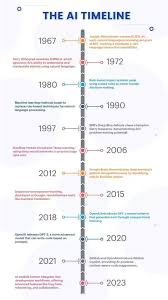
\includegraphics[width=\linewidth]{figures/target-ai-timeline-dense.png}
\caption{T3: ``The AI Timeline'' --- dense vertical infographic, light background, twelve
  year nodes (1967--2023) with colourful connector dots, alternating short bold-year
  + one-sentence blurbs on left/right. (Reference image provided by project owner.)}
\label{fig:target3}
\end{figure}

\paragraph{Visual characterisation.}
\begin{itemize}
  \item \textbf{Layout family:} Vertical central-spine; 12+ year nodes, high density,
        alternating short text blurbs (bold year label + one sentence).
  \item \textbf{Node style:} Small colourful connector dots on the spine, each with a
        distinct accent colour (red, orange, teal, purple, etc.).
  \item \textbf{Content:} Per-node: bold year number as heading; one descriptive sentence.
  \item \textbf{Theme/mood:} Light background, title ``THE AI TIMELINE'' in large uppercase;
        gradient/coloured accents; high information density.
\end{itemize}

\paragraph{Worked Timeline IR.}
Twelve year milestones each carry a one-sentence \texttt{description}. The bold year
label is \texttt{milestone.label}. Per-node colour uses \texttt{category} resolved
through \texttt{theme.category\_map}. The ``dense'' layout mode (tight vertical pitch,
short alternating blurbs) is a render/theme parameter, not IR data.

\begin{lstlisting}[language=yaml,caption={T3 worked IR --- dense AI timeline infographic (abbreviated to four nodes)}]
version: "1.0"
metadata:
  title: "The AI Timeline"
  today: 2026-06-10
  time_range:
    start: 1967-01-01
    end: 2023-12-31
  axis_unit: year
  theme: colorful-infographic     # GAP: theme does not yet exist (Sec. 14.6c)
tracks:
  - id: spine
    label: ""
    index: 0
milestones:
  - id: y1967
    label: "1967"
    date: 1967-01-01
    track: spine
    category: accent-red
    description: "ELIZA demonstrates natural language processing at MIT."
  - id: y1972
    label: "1972"
    date: 1972-01-01
    track: spine
    category: accent-orange
    description: "PROLOG logic programming language is introduced."
  # ... eight further year milestones omitted for brevity ...
  - id: y2015
    label: "2015"
    date: 2015-01-01
    track: spine
    category: accent-blue
    description: "AlphaGo defeats professional Go players for the first time."
  - id: y2023
    label: "2023"
    date: 2023-01-01
    track: spine
    category: accent-purple
    description: "Large language models achieve broad public deployment."
# No activities required: this is a pure milestone spine.
# Per-node colour: theme category_map entry per accent-* category.
# Alternating left/right blurb placement: vertical-spine layout concern.
# Dense pitch: theme parameter (entry_row_height, spine_node_gap).
\end{lstlisting}

\paragraph{IR field mapping summary.}
\texttt{milestones[].label} is the bold year heading.
\texttt{milestones[].description} is the one-sentence blurb.
\texttt{milestones[].category} resolves to node accent colour.
High entry count (12+) is supported without limit; the IR places no cap on list lengths.
All content is expressible. The dense-pitch visual is a theme parameter.

\paragraph{Layout, theme, effects, and tier.}
\begin{itemize}
  \item \textbf{Layout family:} Vertical central-spine with alternating text blurbs
        (same family as T1). \textbf{Gap Render-1} applies.
  \item \textbf{Theme:} Colorful-infographic --- light background, multi-colour
        \texttt{category\_map} entries, bold oversized title, tight spine pitch.
        \textbf{Gap Theme-3}: not in current five themes.
  \item \textbf{Effects:} Gradient/colour accents via \texttt{category\_map} fills;
        no art effects required. Tier~1 (Crisp); SVG backend sufficient.
\end{itemize}


%% ============================================================================
%% T4
%% ============================================================================
\subsection{T4 --- Serpentine Glowing Path}
\label{sec:target-t4}

\begin{figure}[ht]
\centering

\includegraphics[width=\linewidth]{figures/target-serpentine-glow.png}
\caption{T4: Serpentine/winding S-curve path in green with a soft glow--bloom halo;
  milestone dots along the path; a repository-host icon at the start and a clock icon
  (in a ring) at the end. Tier-3 art-effect target. (Reference image provided by project
  owner.)}
\label{fig:target4}
\end{figure}

\paragraph{Visual characterisation.}
\begin{itemize}
  \item \textbf{Layout family:} Serpentine winding path; the time axis is encoded as
        distance along an S-curve, not a straight line. Milestone dots are placed at
        parametric arc positions.
  \item \textbf{Node style:} Small dots along the winding green path; icon at path
        start (repository host pictogram) and end (clock-in-ring pictogram).
  \item \textbf{Art effect:} Prominent soft glow--bloom halo around the entire path;
        rendered via per-pixel compositing (Bloom effect, Raster backend).
  \item \textbf{Theme/mood:} Light background; the path is the hero element; minimal
        supplementary text; ``roadmap as a journey'' metaphor.
\end{itemize}

\paragraph{Worked Timeline IR.}
The milestone positions along the curve are represented by their dates; the serpentine
geometry is the renderer's responsibility. The \texttt{icon} field on boundary milestones
carries pictogram hints. The glow--bloom is declared in the theme's \texttt{fidelity}
block and consumed by the Raster backend.

\begin{lstlisting}[language=yaml,caption={T4 worked IR --- serpentine path (abbreviated)}]
version: "1.0"
metadata:
  title: "Project Roadmap"
  today: 2026-06-10
  time_range:
    start: 2026-01-01
    end: 2026-12-31
  axis_unit: month
  theme: showcase                 # existing Showcase theme (Tier-3 glow supported)
  # GAP: serpentine spine geometry not in Sec. 5 pipeline; see Gap Render-3
tracks:
  - id: journey
    label: ""
    index: 0
milestones:
  - id: start-point
    label: "Project Start"
    date: 2026-01-01
    track: journey
    icon: github-octocat           # pictogram hint: repository host icon
    status: done
  - id: checkpoint-a
    label: "Alpha Release"
    date: 2026-04-01
    track: journey
    status: in-progress
  - id: checkpoint-b
    label: "Beta Release"
    date: 2026-08-01
    track: journey
    status: planned
  - id: end-point
    label: "GA Launch"
    date: 2026-12-01
    track: journey
    icon: clock-ring               # pictogram hint: clock in ring
    status: planned
# GAP Render-3: serpentine spine geometry requires a dedicated module
# (Bezier/spline S-curve); the Sec. 5 straight-axis pipeline does not apply.
# Glow/bloom: Showcase theme fidelity.effects.glow + Bloom; Raster backend.
# Theme category_map: single green fill for path and milestone dots.
\end{lstlisting}

\paragraph{IR field mapping summary.}
\texttt{milestones[].icon} carries the boundary pictogram hints.
\texttt{milestones[].date} positions each dot at its parametric arc position.
\texttt{milestones[].status} drives the dot fill (done/in-progress/planned).
The Bloom effect and glow halo are theme-declared (existing Showcase theme,
Section~\ref{sec:theme-showcase}); the effect registry already contains
\texttt{Bloom\{radius\_px, threshold, intensity, fallback\_policy\}}.
\emph{The sole fundamental gap is the serpentine spine geometry itself.}

\paragraph{Layout, theme, effects, and tier.}
\begin{itemize}
  \item \textbf{Layout family:} Serpentine winding path. \textbf{Gap Render-3} (high
        priority, future scope): requires a new \texttt{spine\_geometry: serpentine}
        layout module with B\'{e}zier/spline S-curve parametrics. This is the most
        architecturally novel layout in the target set and cannot reuse the straight-axis
        pipeline.
  \item \textbf{Theme:} Existing Showcase theme covers glow, bloom, and the Raster
        backend. Only the serpentine geometry is missing from the pipeline.
  \item \textbf{Effects:} Glow (Tier~3 Bloom effect, Raster backend required).
        The \texttt{Bloom} primitive is already defined in the Scene effect registry
        (\S\ref{sec:scene-ir}) and the Showcase theme already activates it. No new
        effect type is needed.
  \item \textbf{Fidelity tier:} Tier~3 (Showcase); Raster backend required for
        per-pixel bloom compositing.
\end{itemize}


%% ============================================================================
%% T5
%% ============================================================================
\subsection{T5 --- Gitline: Card Timeline, Dark Textured, Data-Driven}
\label{sec:target-t5}

\begin{figure}[ht]
\centering
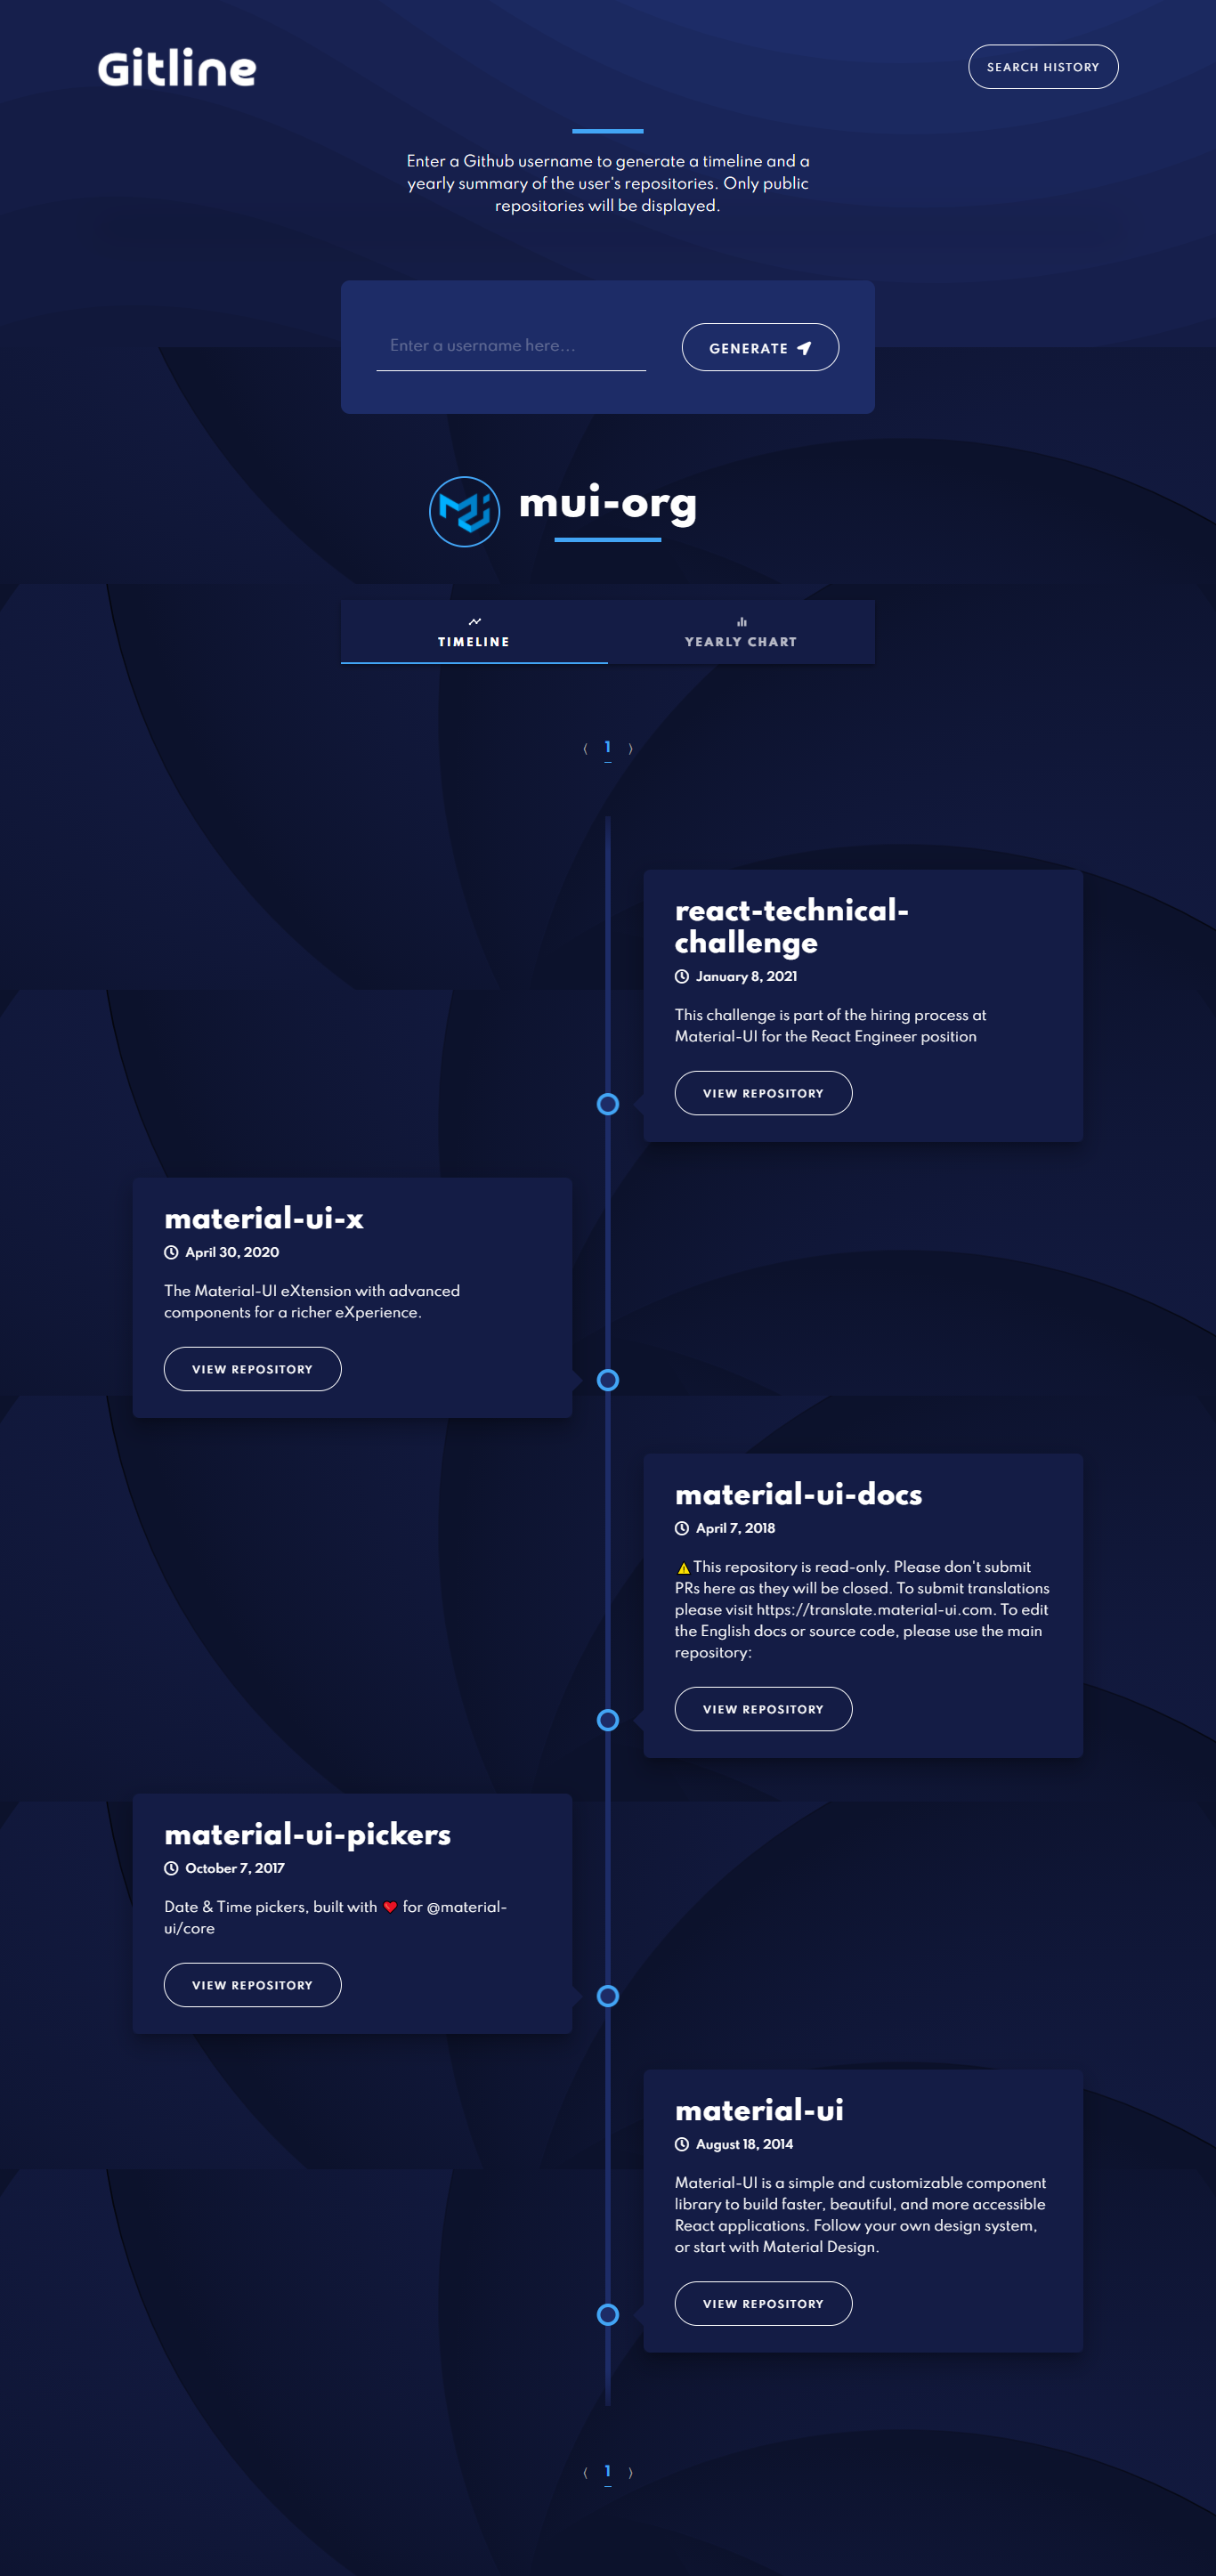
\includegraphics[width=0.85\linewidth]{figures/target-gitline-cards.png}
\caption{T5: Gitline web app --- dark navy background with subtle swirl/radial texture;
  vertical central spine; alternating rounded cards (bold repo title, clock-icon date,
  description paragraph, ``VIEW REPOSITORY'' CTA button); one card with a warning callout;
  org header with avatar; TIMELINE / YEARLY CHART tabs; pagination. (Reference image
  provided by project owner.)}
\label{fig:target5}
\end{figure}

\paragraph{Visual characterisation.}
\begin{itemize}
  \item \textbf{Layout family:} Vertical central-spine with alternating rounded cards;
        same family as T1 and T3.
  \item \textbf{Card anatomy:} Bold repo title (activity label), date with clock icon
        (activity start), description paragraph, ``VIEW REPOSITORY'' outline CTA button
        (activity url). One card carries a small warning note.
  \item \textbf{Data source:} GitHub username/org input drives activity generation
        (this is the project's core data-ingestion flow; the IR result is independent
        of the source).
  \item \textbf{Theme/mood:} Dark navy background (\texttt{\#0D1117} range), subtle
        swirl/radial background texture (Tier-3 art effect), rounded cards with soft
        border--shadow, pagination control.
  \item \textbf{Alternate view:} A ``YEARLY CHART'' tab shows the same IR data in a
        histogram/chart layout --- a separate render target, not a different IR.
\end{itemize}

\paragraph{Worked Timeline IR.}
Repository entries map directly to \texttt{activities}. The ``VIEW REPOSITORY'' CTA uses
\texttt{activity.url} (already in the IR schema). The warning note maps to an
\texttt{annotations} callout. The org avatar and web UI chrome (search input, tabs,
pagination) are render/shell concerns, not IR data. The dark textured background is
declared in the theme's \texttt{fidelity} block (Showcase dark variant).

\begin{lstlisting}[language=yaml,caption={T5 worked IR --- Gitline card timeline (abbreviated)}]
version: "1.0"
metadata:
  title: "Gitline: mui-org"
  author: "mui-org"
  today: 2026-06-10
  time_range:
    start: 2020-06
    end: 2022-06
  axis_unit: month
  theme: showcase-dark            # GAP: dark variant of Showcase (Sec. 14.6c)
  description: "Repository timeline for the mui-org GitHub organisation"
tracks:
  - id: repos
    label: "Repositories"
    index: 0
activities:
  - id: react-tech-challenge
    label: "react-technical-challenge"
    track: repos
    span: 2021-01
    description: "A technical challenge project for React developers."
    url: "https://github.com/mui-org/react-technical-challenge"
    status: done
    category: repo-card
  - id: material-ui-v5
    label: "material-ui v5"
    track: repos
    start: 2021-03
    end: 2021-09
    description: "Major version release with full redesign of component APIs."
    url: "https://github.com/mui-org/material-ui"
    status: done
    category: repo-card
  - id: mui-x-grid
    label: "mui-x-grid"
    track: repos
    start: 2021-06
    end: 2022-01
    description: "Advanced data grid component with enterprise features."
    url: "https://github.com/mui-org/mui-x"
    status: in-progress
    category: repo-card
annotations:
  - type: callout
    target: react-tech-challenge
    text: "Repository archived; no recent commits since 2021."
    style: warning                # theme maps 'warning' to amber callout style
# activity.url --> "VIEW REPOSITORY" CTA button (renderer generates button label)
# Org avatar header: theme asset / web-app shell; not IR data
# YEARLY CHART tab: alternate render of the same IR; no IR schema change needed
# Swirl background texture: theme fidelity.effects.noise_texture (Tier-3 Raster)
# Pagination: HTML backend concern; no IR field needed
\end{lstlisting}

\paragraph{IR field mapping summary.}
\texttt{activities[].label} is the bold card title.
\texttt{activities[].start} / \texttt{span} renders as the clock-icon date.
\texttt{activities[].description} is the card body paragraph.
\texttt{activities[].url} is the ``VIEW REPOSITORY'' CTA link target; the button label
is a theme-level string constant (render concern, not IR data).
\texttt{annotations[].style: warning} maps to the warning callout via
\texttt{theme.annotation} styling.
The ``YEARLY CHART'' alternate view is a second render pass on the same IR document
with a different \texttt{spine\_geometry} or chart backend---no IR change required.

\paragraph{Layout, theme, effects, and tier.}
\begin{itemize}
  \item \textbf{Layout family:} Vertical central-spine with alternating rounded cards.
        \textbf{Gap Render-1} applies (same as T1/T3). Additionally, the card rendering
        anatomy (title--date--description--CTA-button within a rounded-rect card shape)
        requires a dedicated card-entry renderer. \textbf{Gap Render-4.}
  \item \textbf{Theme:} Showcase dark variant --- deep navy background, swirl/radial
        texture via \texttt{noise\_texture} / \texttt{cloud\_layer} effects, rounded
        card shapes with soft borders and shadows.
        \textbf{Gap Theme-4}: the existing Showcase theme has a dark palette option
        (\texttt{\#0A1628} background) but does not define card-entry shape rendering
        or the CTA-button primitive. A \texttt{showcase-dark} child theme is needed.
  \item \textbf{Effects:} Background swirl/radial texture (\texttt{NoiseTexture} or
        \texttt{CloudLayer}, Tier~3); drop shadows on cards (Tier~2 \texttt{DropShadow},
        already in effect registry). Raster backend required for the texture layer;
        SVG backend handles card geometry with \texttt{embed-raster} fallback for texture.
  \item \textbf{Fidelity tier:} Tier~3 (Showcase); Raster backend required for
        background texture; HTML backend for interactive CTA links and pagination.
\end{itemize}


%% ============================================================================
%% SYNTHESIS
%% ============================================================================
\subsection{Synthesis}
\label{sec:target-synthesis}

\subsubsection{A: Layout Families Finding}
\label{sec:target-layout-families}

The current \S5 rendering model implements a single layout family: \textbf{horizontal
swimlane Gantt} (orientation: horizontal; spine geometry: straight; entry placement:
parallel track bands). The five targets expose three additional families:

\begin{enumerate}
  \item \textbf{Vertical central-spine with alternating entries} (T1, T3, T5):
        orientation rotated 90\textdegree; a single central line runs top-to-bottom;
        entries (text blurbs, subject headings, or rounded cards) alternate left and
        right of year/date nodes; icon badges may anchor at the canvas edges with leader
        lines.

  \item \textbf{Horizontal single-line with numbered nodes} (T2):
        orientation horizontal; but the track-band structure is collapsed to a single
        zero-height line; milestones are rendered as large numbered circles; date appears
        above the node, title below; no activity bars. This is an edge case of the
        existing pipeline achievable by suppressing the track header column and axis band
        and overriding the milestone shape---no separate layout engine is strictly
        required, but the milestone geometry (Phase~4, \S\ref{sec:phase4}) needs a
        ``numbered circle'' shape variant.

  \item \textbf{Serpentine winding path} (T4):
        spine geometry is a parametric B\'{e}zier S-curve; time is encoded as arc-length
        position along the curve; the date-to-coordinate function $x(T)$ is replaced by
        a curve parametrisation $\mathbf{p}(t(T))$. This is architecturally the most
        novel family and cannot share Phase~1--6 geometry with the straight-axis pipeline.
\end{enumerate}

\paragraph{Layout family is a render/theme concern; the IR stays layout-agnostic.}
The Timeline IR (\S4) makes no assumption about axis orientation or spine geometry.
Field semantics (\texttt{date}, \texttt{track}, \texttt{milestones}) are spatial only
in the sense that a renderer maps them to a canvas. Swapping layout family requires
only a theme/renderer change; the same IR document is valid for any family.

\paragraph{Recommendation.}
Add an explicit \texttt{layout\_family} property to the \emph{theme schema}
(Section~\ref{sec:themes-schema}) with the structure:

\begin{itemize}
  \item \texttt{orientation}: \texttt{horizontal} (default) $|$ \texttt{vertical}
  \item \texttt{spine\_geometry}: \texttt{straight} (default) $|$ \texttt{serpentine}
  \item \texttt{entry\_placement}: \texttt{swimlane} (default) $|$ \texttt{alternating}
        $|$ \texttt{card} $|$ \texttt{numbered-single-line}
\end{itemize}

This property lives in the theme, not the IR. The layout engine dispatches to the
appropriate Phase-1--6 pipeline variant based on \texttt{layout\_family.orientation}
and \texttt{spine\_geometry}. The IR contract is unchanged.

\subsubsection{B: Consolidated Coverage Table}
\label{sec:target-coverage-table}

\begin{table}[ht]
\centering
\footnotesize
\begin{tabularx}{\textwidth}{lXXXXX}
\toprule
\textbf{Target} &
\textbf{IR-Expressible?} &
\textbf{Layout Family Supported?} &
\textbf{Theme Available?} &
\textbf{Effects / Tier} &
\textbf{Notes} \\
\midrule
T1 Vertical spine, dark &
Partial &
No &
No &
Tier~2 (DropShadow) &
Vertical-spine layout gap; dark-executive theme gap; icon-badge leader-line render gap;
per-node colour via \texttt{category\_map} workaround \\[4pt]

T2 Horizontal numbered &
Yes &
Partial &
Partial &
Tier~1 (Crisp) &
Data fully representable; numbered-circle node shape not in current milestone geometry;
light-minimal-corporate theme variant needed \\[4pt]

T3 Dense AI infographic &
Yes &
No &
No &
Tier~1 (Crisp) &
All data via \texttt{milestones[].description + category}; vertical-spine layout gap;
colorful-infographic theme gap \\[4pt]

T4 Serpentine glow &
Partial &
No &
Partial &
Tier~3 (Bloom, Raster) &
Data representable; serpentine spine geometry is fundamental layout gap;
Showcase theme covers glow/bloom effect \\[4pt]

T5 Gitline cards, dark &
Yes &
No &
Partial &
Tier~3 (NoiseTexture + DropShadow) &
\texttt{activity.url} covers CTA link; \texttt{annotation.callout} covers warning;
vertical-spine + card-entry render gap; showcase-dark theme variant gap \\
\bottomrule
\end{tabularx}
\caption{Coverage analysis: five targets versus current design (IR, layout, theme, effects)}
\label{tab:target-coverage}
\end{table}


\subsubsection{C: Gap List}
\label{sec:target-gap-list}

\paragraph{(a) IR gaps --- flagged for Mark (Section~\ref{sec:ir})}
\label{sec:target-gaps-ir}

\begin{description}
  \item[IR-1: Milestones lack \texttt{metadata} extension field.]
        Activities carry \texttt{metadata: map<string,any>} for arbitrary render hints
        and extension data; milestones do not. As T1 and T3 show, milestones (year nodes)
        are the primary semantic entity in infographic layouts and benefit equally from
        open extension. Workaround: \texttt{tags: [list<string>]} can carry string flags
        but not structured key--value data.
        \emph{Recommendation for Mark: add \texttt{metadata: map<string,any>} to the
        Milestone schema.}

  \item[IR-2: Activities and milestones lack a direct \texttt{color} field.]
        Neither entity type has \texttt{color: string?} (tracks do). Per-entity colour
        today requires defining a separate \texttt{category} and a corresponding
        \texttt{category\_map} entry in the theme. For dense infographic layouts (T1: 4
        year colours; T3: 12 accent colours) this is ergonomically burdensome: 12 theme
        category definitions just to express 12 distinct dot colours. The \texttt{color}
        hint on tracks shows the precedent.
        \emph{Recommendation for Mark: add \texttt{color: string?} to Activity and
        Milestone (as a direct colour override hint, applied after \texttt{category\_map}
        and before \texttt{status\_map}).}

  \item[IR-3: \texttt{annotation.callout} has no \texttt{icon} field.]
        In T1, the circular icon badge at the canvas edge is semantically ``the
        milestone's icon rendered in a badge callout''. The current design resolves this
        by having the vertical-spine layout module read \texttt{milestone.icon} and
        auto-generate the badge---no separate annotation or IR change is needed. Confirmed
        not an IR gap; documented for clarity.

  \item[IR-4: Multiple subjects under one year node.]
        T1 shows two stacked subjects under 2023. Representable today via
        \texttt{groups[].members} containing two activities both with \texttt{span: 2023}.
        The renderer clusters group members at the same node. Confirmed not an IR gap.

  \item[IR-5: CTA link label is not separately stored.]
        T5's ``VIEW REPOSITORY'' button text is not in the IR; the renderer uses a
        theme-level default label derived from \texttt{activity.url}. Authors who want a
        custom CTA label can use \texttt{activity.metadata.cta\_label: "..."}. No IR
        schema change needed; documented for theme implementers.
\end{description}

\paragraph{(b) Render and layout additions --- owned by Barbara}

\begin{description}
  \item[Render-1: Vertical central-spine layout module (Priority 1).]
        Covers T1, T3, T5 (three of five targets). New \texttt{layout\_family} property
        in the theme schema (\texttt{orientation: vertical},
        \texttt{entry\_placement: alternating | card}). The Phase-1 axis computation
        maps dates to the $y$-axis; Phases 2--4 compute entry positions left/right of
        the spine. The Phase-1--6 pipeline structure is preserved; phases are
        parameterised, not replaced.

  \item[Render-2: Numbered circular node shape for milestones (Priority 2).]
        Covers T2. A new milestone shape variant \texttt{shape: numbered-circle} in the
        theme \texttt{milestone} block. The renderer assigns ordinal numbers by
        milestone sort order; no IR field needed.

  \item[Render-3: Serpentine spine geometry (Priority 3 / future scope).]
        Covers T4. Replaces the straight-axis date-to-coordinate function with a
        parametric B\'{e}zier S-curve module. The date-to-arc-length mapping must be
        monotone and deterministic. Architecturally the most complex addition; recommended
        for a post-MVP release.

  \item[Render-4: Card-entry rendering for vertical-spine (Priority 2).]
        Covers T5. Within the vertical-spine layout, entries rendered as rounded-rect
        cards (title text, date--icon row, description paragraph, CTA-button primitive).
        The card shape and CTA-button are theme-defined; data comes from
        \texttt{activity.\{label, start, description, url\}}.

  \item[Render-5: Dashed-leader annotation connector style (Priority 2).]
        Covers T1 icon-badge leader lines. Extend the
        \texttt{theme.annotation.connector\_style} vocabulary with
        \texttt{dashed-leader-arrow} (dashed stroke with arrowhead terminus). The
        annotation \texttt{type: connector} is already in the IR; only the visual
        style is missing.

  \item[Render-6: ``YEARLY CHART'' alternate view (out of scope / future).]
        Covers T5 tab. A chart/histogram render pass on the same IR; not in scope
        for the Timeline Compiler's timeline rendering mandate. Deferred.
\end{description}

\paragraph{(c) Theme additions --- owned by Barbara}
\label{sec:target-gaps-theme}

\begin{description}
  \item[Theme-1: \texttt{dark-executive} (Priority 1).]
        Deep charcoal--navy background, coloured spine segments per category, drop-shadow
        icon badges, clean sans-serif. Fidelity Tier~2. Maps to T1 (dark spine, year
        nodes) and the dark shell of T5 (Gitline). Extends the existing Showcase base:
        \texttt{extends: showcase}; overrides \texttt{canvas.background\_color},
        \texttt{layout\_family.orientation: vertical}, \texttt{fidelity.tier: 2}.

  \item[Theme-2: \texttt{light-minimal-corporate} (Priority 2).]
        White background, generous whitespace, numbered circular milestone nodes, no
        gridlines, large milestone labels. Fidelity Tier~1. Maps to T2. Extends
        Consulting: \texttt{extends: consulting}; overrides
        \texttt{milestone.shape: numbered-circle},
        \texttt{layout\_family.entry\_placement: numbered-single-line}.

  \item[Theme-3: \texttt{colorful-infographic} (Priority 2).]
        Light background, multi-accent \texttt{category\_map} (12 colours pre-defined),
        dense vertical pitch (tight \texttt{spine\_node\_gap}), bold oversized title
        typography. Fidelity Tier~1. Maps to T3. New standalone theme; no suitable
        parent among the current five.

  \item[Theme-4: \texttt{showcase-dark} child theme (Priority 1).]
        Extends \texttt{showcase}; overrides background to deep navy (\texttt{\#0D1117}),
        activates \texttt{noise\_texture} effect (swirl/radial), sets
        \texttt{layout\_family.orientation: vertical},
        \texttt{layout\_family.entry\_placement: card}. Maps to T5 Gitline aesthetic.
        Fidelity Tier~3; Raster backend required for texture; HTML backend for
        interactive CTA links.
\end{description}

\paragraph{(d) Effects validation against effect registry}

All effects required by the five targets are already defined in the Scene effect registry
(\S\ref{sec:scene-ir}) and theme fidelity schema (\S\ref{sec:schema-fidelity}):

\begin{itemize}
  \item \textbf{Glow / Bloom (T4)}: \texttt{Bloom\{radius\_px, threshold, intensity,
        fallback\_policy\}} and \texttt{Glow\{color, radius\_px, intensity\}} are
        registered effects. Showcase theme activates them. Raster backend renders
        per-pixel; SVG backend emits \texttt{feGaussianBlur+feComposite} with
        determinism caveat; PPTX maps to native \texttt{a:glow}.

  \item \textbf{Background swirl texture (T5)}: \texttt{NoiseTexture\{seed, scale,
        turbulence\_type, opacity\}} and \texttt{CloudLayer\{seed, scale, octaves,
        opacity, color\_stops\}} are both registered. The seed is derived from
        \texttt{scene\_hash + effect\_id} (deterministic). Raster backend renders
        natively; SVG backend applies \texttt{embed-raster} fallback policy.

  \item \textbf{Drop shadows (T1, T5)}: \texttt{DropShadow\{offset\_x, offset\_y,
        blur\_radius, color, opacity, fallback\_policy\}} is registered and active in
        the Showcase theme. PPTX maps to native \texttt{a:outerShdw}; SVG backend uses
        \texttt{feDropShadow} with determinism caveat at Tier~2.

  \item \textbf{Dashed-leader connector style (T1)}: This is a \emph{stroke style}
        extension on the existing \texttt{Line} Scene primitive (the annotation
        connector), not a new effect type. Add \texttt{dashed-leader-arrow} to the
        \texttt{theme.annotation.connector\_style} vocabulary. No new Scene effect
        definition required.
\end{itemize}

\subsubsection{D: Verdict}
\label{sec:target-verdict}

The Timeline IR can already represent the \emph{data content} of all five targets
without schema changes, with two exceptions flagged for Mark: the missing
\texttt{metadata} field on \texttt{Milestone} (Gap IR-1) and the absence of a direct
\texttt{color} hint on \texttt{Activity} and \texttt{Milestone} (Gap IR-2).
All other requirements are render, layout, theme, or effect concerns that Barbara owns.

The current render--theme architecture \emph{can} produce all five targets given the
following additions, in priority order:

\begin{enumerate}
  \item \textbf{Vertical central-spine layout family} (Render-1): unlocks T1, T3, T5
        simultaneously; highest return on investment.
  \item \textbf{Dark-executive theme} (Theme-1) and \textbf{showcase-dark child theme}
        (Theme-4): cover T1 and T5 dark aesthetics.
  \item \textbf{Card-entry renderer} (Render-4) and \textbf{numbered-circle milestone
        shape} (Render-2): complete T5 and T2 respectively.
  \item \textbf{Light-minimal-corporate} (Theme-2) and
        \textbf{colorful-infographic} (Theme-3) themes: complete T2 and T3.
  \item \textbf{Dashed-leader connector style} (Render-5): completes T1 icon callout
        fidelity.
  \item \textbf{Serpentine layout module} (Render-3): completes T4; recommended for
        a post-MVP release given its architectural novelty.
\end{enumerate}

The effect infrastructure (glow, bloom, drop shadow, noise texture, cloud layer) is
\emph{already designed and sufficient}. No new Scene effect types are required.
The fidelity-tier and backend model (\S\ref{sec:fidelity-tiers}) correctly classifies
T4 and T5 as Tier~3 (Raster backend required) and T1--T3 as Tier~1--2 (SVG backend
sufficient). The design is sound; the gap is in the layout family and theme inventory,
not in the core architecture.
